% Copyright 2004 by Till Tantau <tantau@users.sourceforge.net>.
%
% In principle, this file can be redistributed and/or modified under
% the terms of the GNU Public License, version 2.
%
% However, this file is supposed to be a template to be modified
% for your own needs. For this reason, if you use this file as a
% template and not specifically distribute it as part of a another
% package/program, I grant the extra permission to freely copy and
% modify this file as you see fit and even to delete this copyright
% notice. 

\documentclass{beamer}

\usepackage{blindtext}
\usepackage{tcolorbox}

\usefonttheme{professionalfonts} % using non standard fonts for beamer
\usefonttheme{serif} % default family is serif
%\usepackage{fontspec}
%\setmainfont{Liberation Serif}

% There are many different themes available for Beamer. A comprehensive
% list with examples is given here:
% http://deic.uab.es/~iblanes/beamer_gallery/index_by_theme.html
% You can uncomment the themes below if you would like to use a different
% one:
%\usetheme{AnnArbor}
%\usetheme{Antibes}
%\usetheme{Bergen}
%\usetheme{Berkeley}
%\usetheme{Berlin}
%\usetheme{Boadilla}
%\usetheme{boxes}
%\usetheme{CambridgeUS}
%\usetheme{Copenhagen}
%\usetheme{Darmstadt}
\usetheme{default}
%\usetheme{Frankfurt}
%\usetheme{Goettingen}
%\usetheme{Hannover}
%\usetheme{Ilmenau}
%\usetheme{JuanLesPins}
%\usetheme{Luebeck}
%\usetheme{Madrid}
%\usetheme{Malmoe}
%\usetheme{Marburg}
%\usetheme{Montpellier}
%\usetheme{PaloAlto}
%\usetheme{Pittsburgh}
%\usetheme{Rochester}
%\usetheme{Singapore}
%\usetheme{Szeged}
%\usetheme{Warsaw}



\title{Digital Signal Processing: Theory and Practice}

% A subtitle is optional and this may be deleted
\subtitle{}

\author{Sivakumar Balasubramanian}
% - Give the names in the same order as the appear in the paper.
% - Use the \inst{?} command only if the authors have different
%   affiliation.

\institute[Christian Medical College] % (optional, but mostly needed)
{
  \inst{}%
  Department of Bioengineering\\
  Christian Medical College, Bagayam\\
  Vellore 632002
}
% - Use the \inst command only if there are several affiliations.
% - Keep it simple, no one is interested in your street address.

\date{}
% - Either use conference name or its abbreviation.
% - Not really informative to the audience, more for people (including
%   yourself) who are reading the slides online

\subject{Lecture notes on signal processing}
% This is only inserted into the PDF information catalog. Can be left
% out. 

% If you have a file called "university-logo-filename.xxx", where xxx
% is a graphic format that can be processed by latex or pdflatex,
% resp., then you can add a logo as follows:

% \pgfdeclareimage[height=0.5cm]{university-logo}{university-logo-filename}
% \logo{\pgfuseimage{university-logo}}

% Delete this, if you do not want the table of contents to pop up at
% the beginning of each subsection:
\AtBeginSubsection[]
{
  \begin{frame}<beamer>{Outline}
    \tableofcontents[currentsection,currentsubsection]
  \end{frame}
}

% Let's get started
\begin{document}

\begin{frame}
  \titlepage
\end{frame}

% WHAT IS SIGNAL PROCESSING?
\begin{frame}{What is signal processing?}
\textit{
"Signal processing is an enabling technology that encompasses the fundamental theory, applications, algorithms, and implementations of \textbf{processing or transferring information} contained in many different physical, symbolic, or abstract formats broadly designated as signals and uses \textbf{mathematical, statistical, computational, heuristic, and/or linguistic representations}, formalisms, and techniques for \textbf{representation, modeling, analysis, synthesis, discovery, recovery, sensing, acquisition, extraction, learning, security, or forensics}."}\footnote{\tiny{Moura, J.M.F. (2009). "What is signal processing?, President’s Message". IEEE Signal Processing Magazine 26 (6). doi:10.1109/MSP.2009.934636}}
\end{frame}

% WHAT IS A SIGNAL?
\begin{frame}{What is a signal?}

Any physical quantity carrying information that varies with one or more independent variables.
$$ s\left(t\right) = 1.23t^2 - 5.11t +41.5 $$
$$ s\left(x,y\right) = e^{-(x^2 + y^2 + 0.5xy)} $$

Mathematical representation will not be possible (e.g. \textit{physiological signals,  either because the exact function is not known or is too complicated}.)
\end{frame}

% WHAT IS A SIGNAL?
\begin{frame}{What is a signal? (Contd ... )}

\begin{figure}
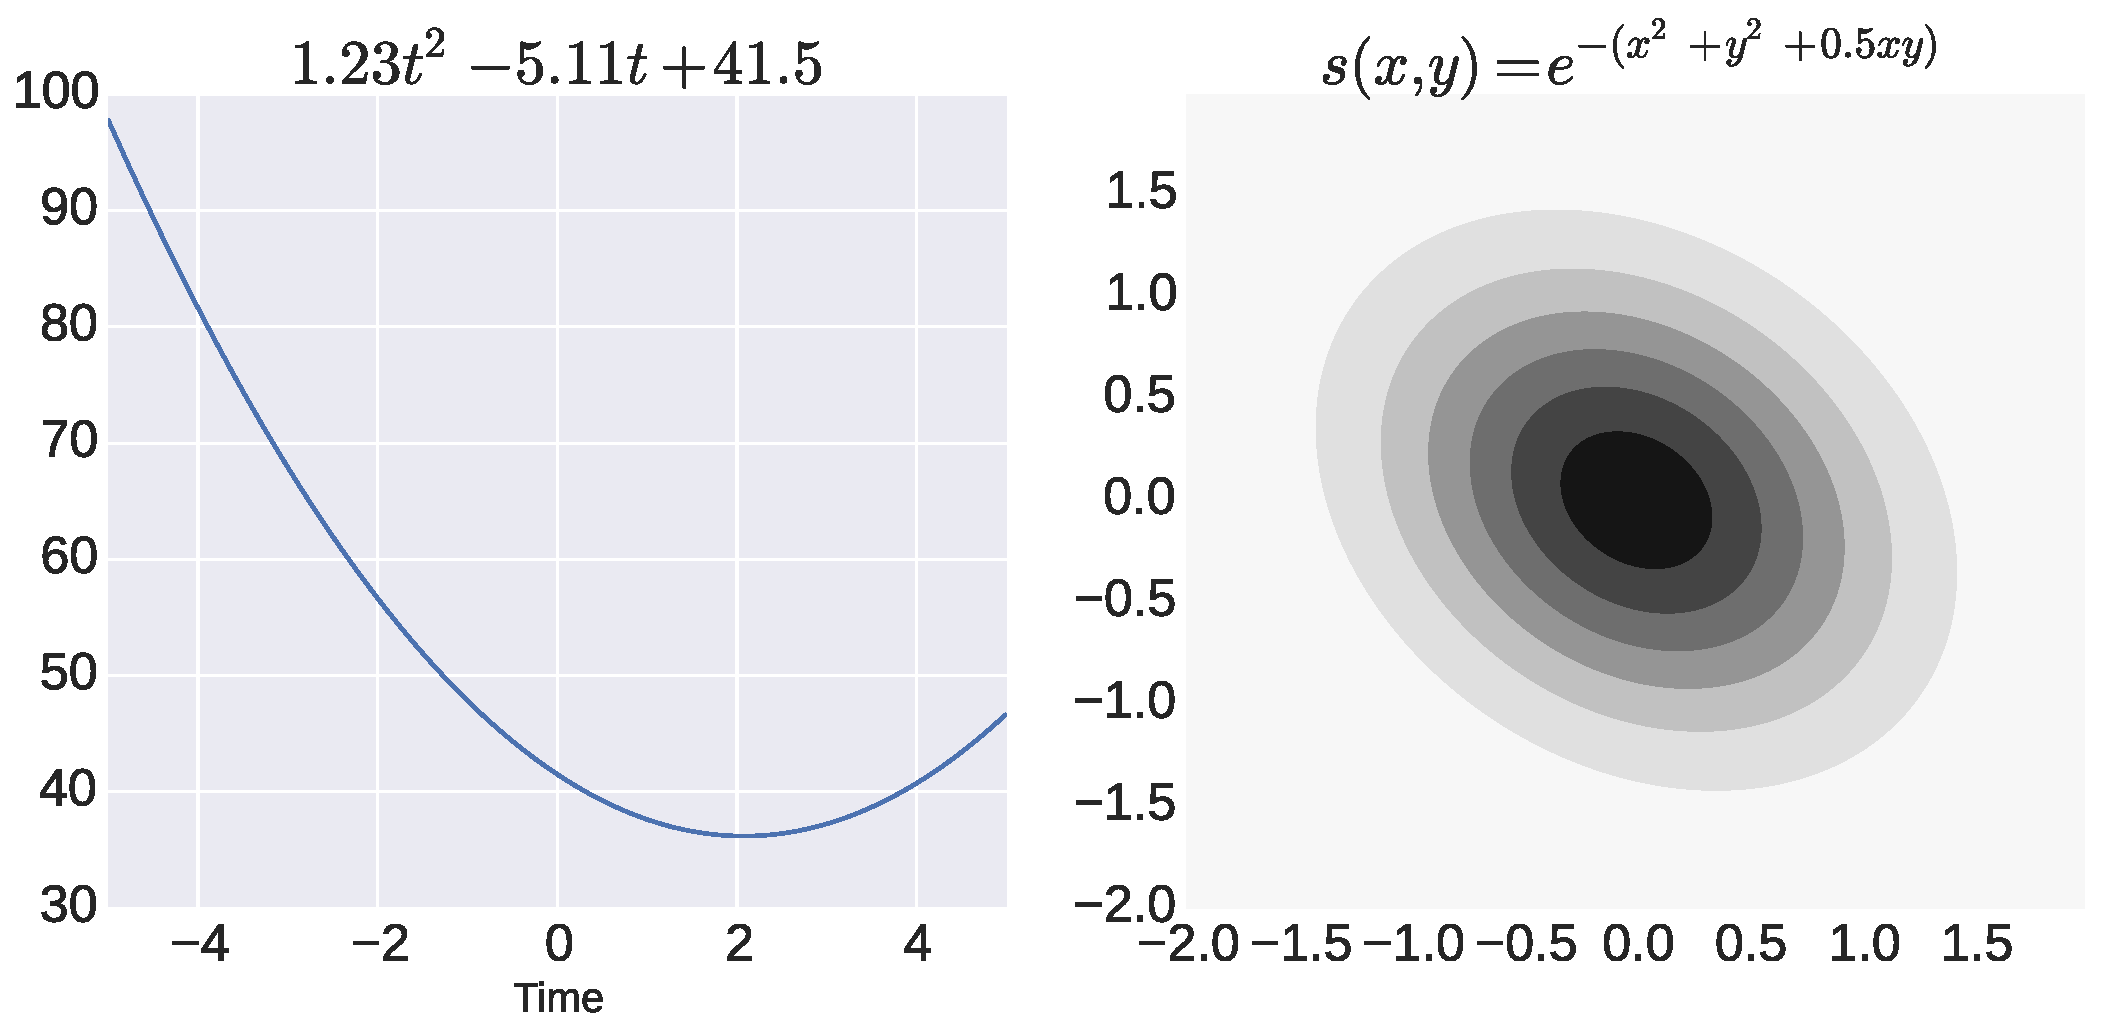
\includegraphics[width=\textwidth]{img/signals.eps}
\caption{Example of 1D and 2D signals}
\end{figure}

\textit{Can you think of examples of 3D and 4D signals?}
\end{frame}

% WHAT IS A SIGNAL?
\begin{frame}{What is a signal?}

Any physical quantity carrying information that varies with one or more independent variables.
$$ s\left(t\right) = 1.23t^2 - 5.11t +41.5 $$
$$ s\left(x,y\right) = e^{-(x^2 + y^2 + 0.5xy)} $$

Mathematical representation will not be possible (e.g. \textit{physiological signals,  either because the exact function is not known or is too complicated}.)
\end{frame}

% CLASSIFICATION OF SIGNALS
\begin{frame}{Classification of signals}\
\begin{itemize}
\item Based on the signal dimensions. \textit{e.g.} 1D, 2D ...
\item \textbf{Scalar} vs. \textbf{Vector} signals: \textit{e.g. gray scale versus RGB image}
\[I_g\left(x,y\right) \in \mathbb{R} \,\,\mathrm{and}\,\, I_{color}\left(x,y\right) \in \mathbb{R}^3\]
\item \textbf{Continuous-time} vs. \textbf{Discrete-time}: \textit{based on the values assumed by the independent variable.}
\[
\begin{cases}
x(t) = e^{-0.1t^{2}}, \,\, t \in \mathbb{R} & \text{Continuous-time} \\
x[n] = e^{-0.1n^{2}}, \,\, n \in \mathbb{Z} & \text{Discrete-time}
\end{cases}
 \]
\end{itemize}
\begin{figure}
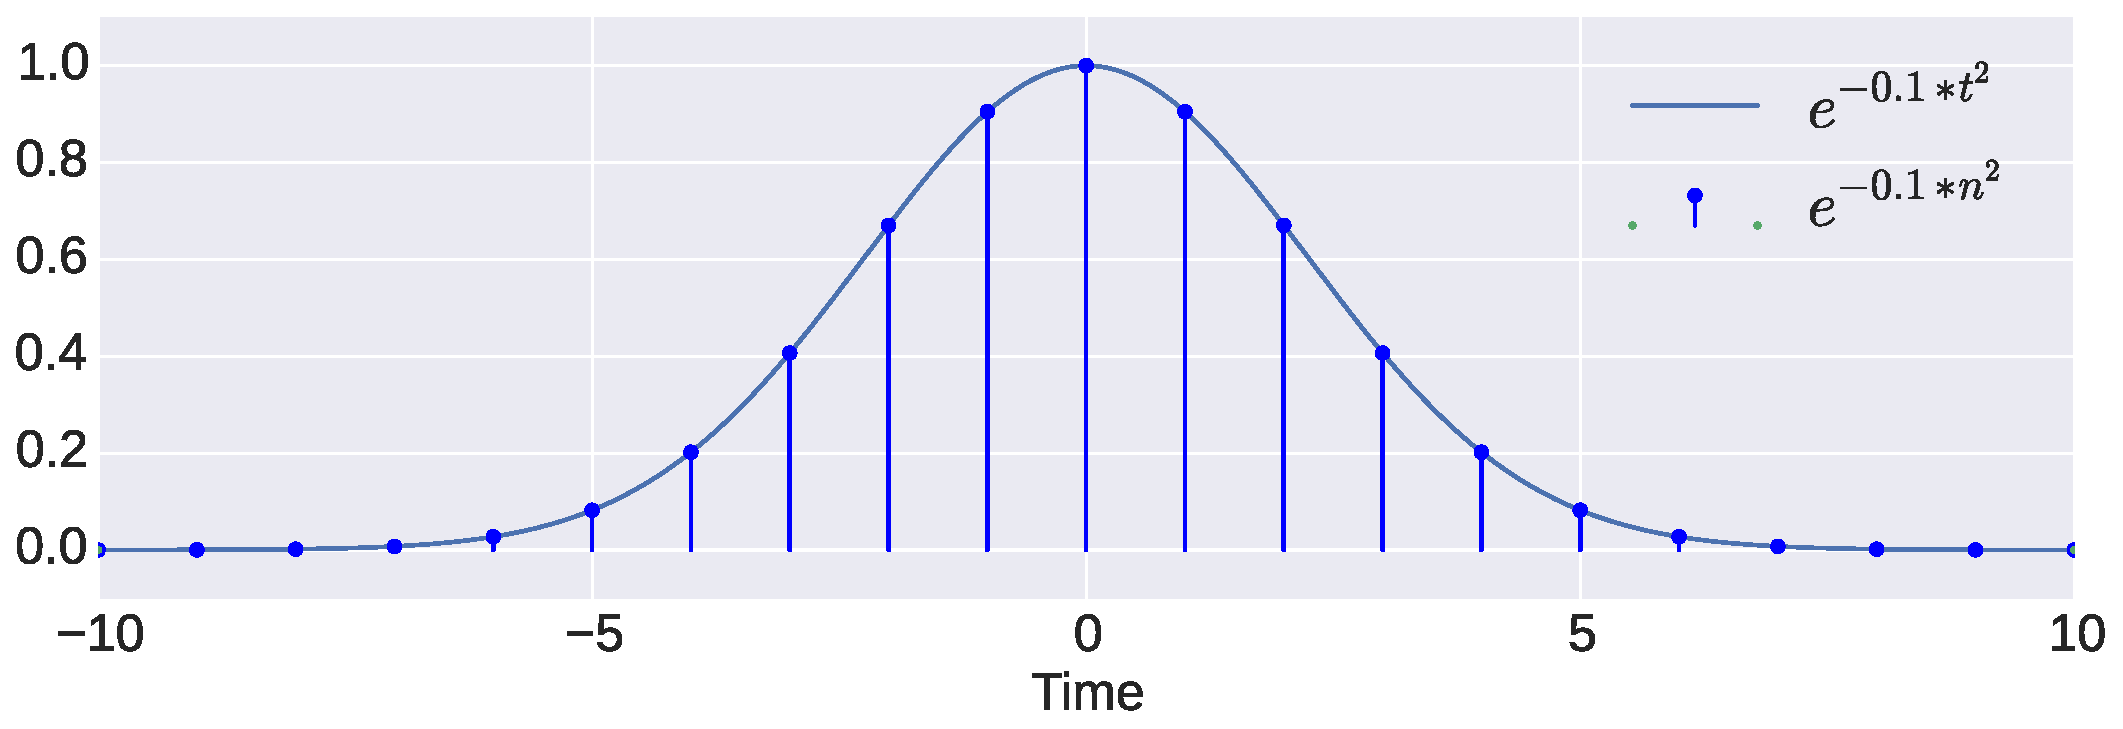
\includegraphics[width=0.8\textwidth]{img/cont_disc.eps}
\end{figure}
\end{frame}

% CLASSIFICATION OF SIGNALS
\begin{frame}{Classification of signals (Contd ...)}
\begin{itemize}
\item \textbf{Continuous-valued} vs. \textbf{Discrete-valued}: \textit{based on the values assumed by the dependent variable.}
\[
\begin{cases}
x(t) \in [a, b] & \text{Continuous-valued} \\
x(t) \in \{a_1, a_2, \cdots\} & \text{Discrete-valued} \\
\end{cases}
 \]
\end{itemize}
\begin{figure}
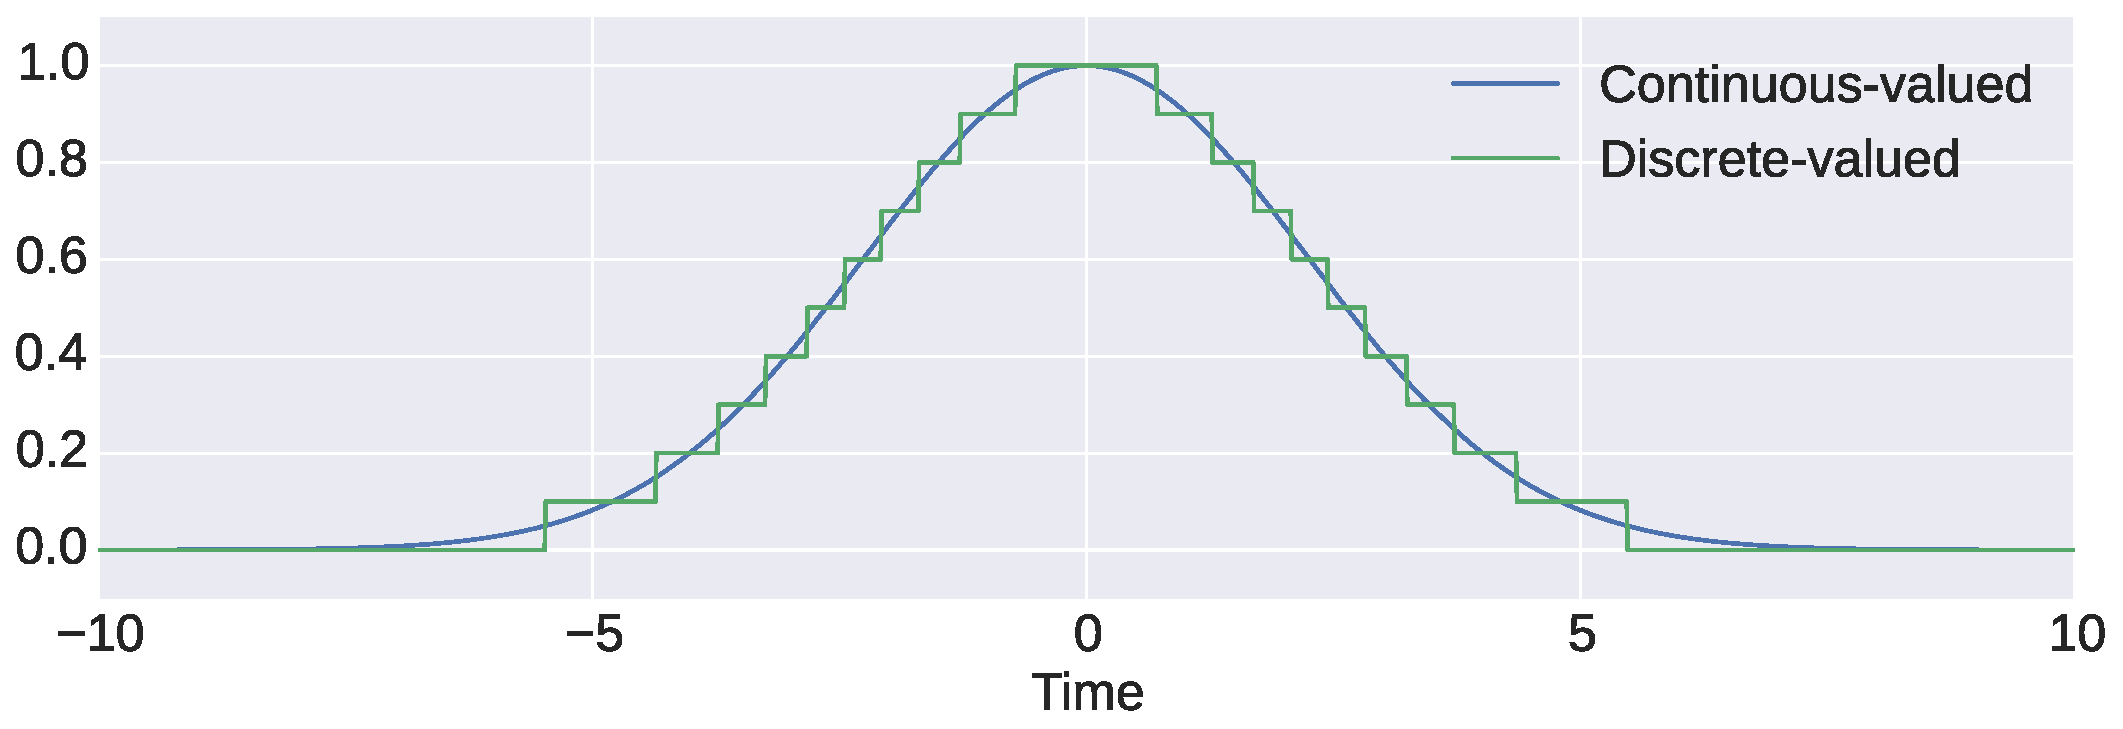
\includegraphics[width=0.8\textwidth]{img/cont_disc_val.eps}
\end{figure}
\end{frame}

% CLASSIFICATION OF SIGNALS
\begin{frame}{Classification of signals (Contd ...)}
\textbf{Four types of signals}
\begin{figure}
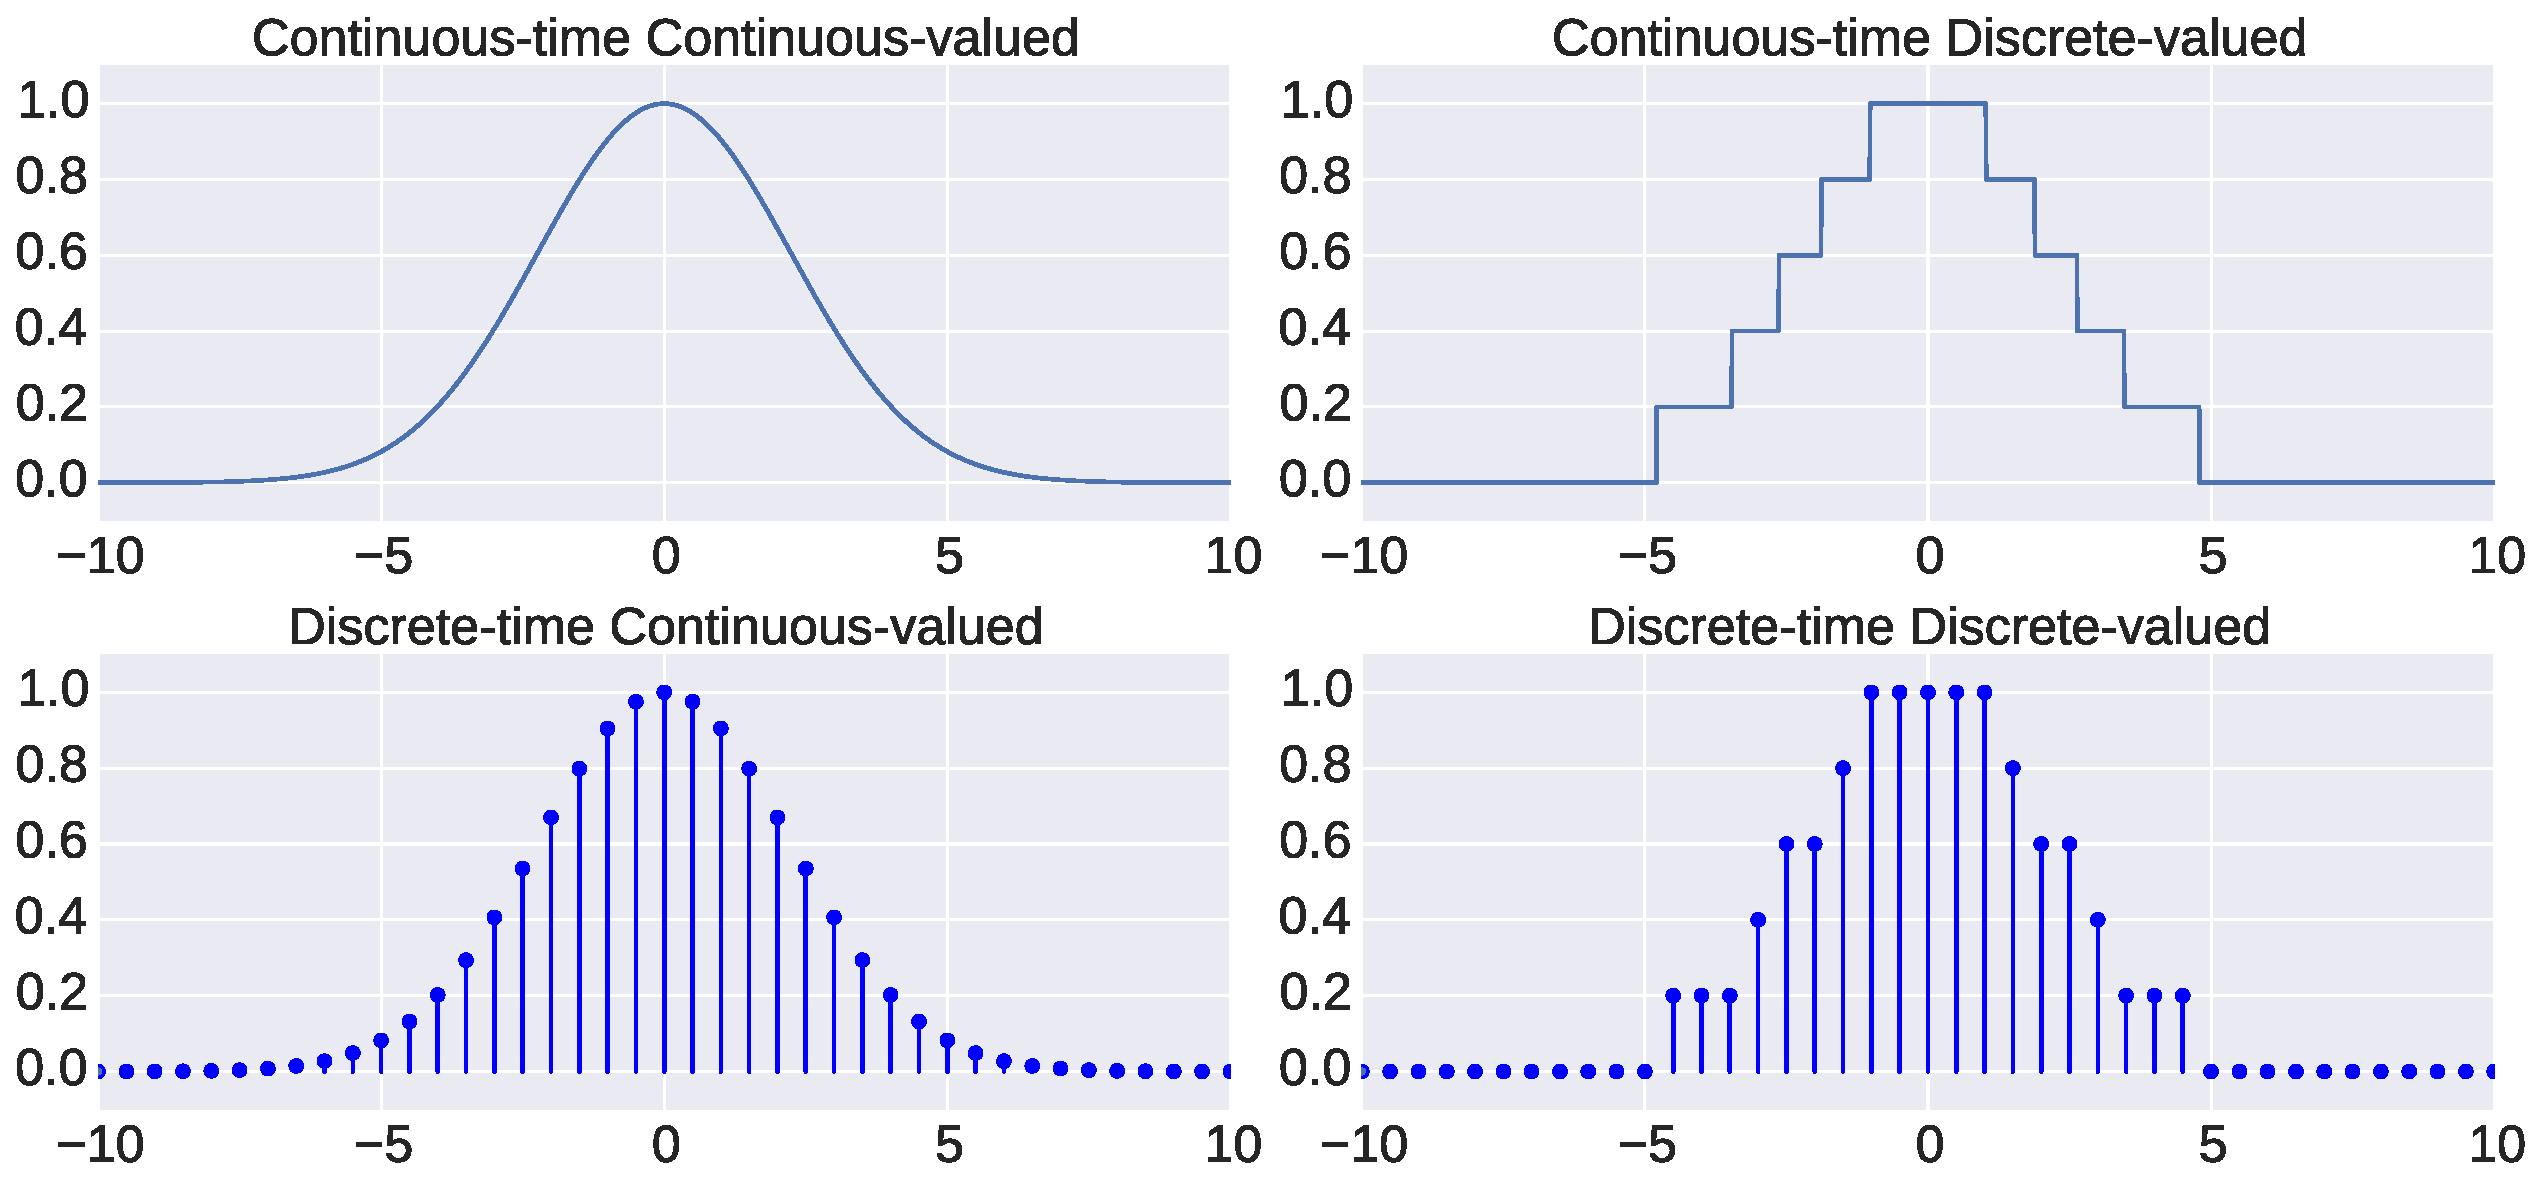
\includegraphics[width=\textwidth]{img/signal_types.eps}
\end{figure}
\end{frame}

% CLASSIFICATION OF SIGNALS
\begin{frame}{Classification of signals (Contd ...)}
\textbf{Example of a Continuous-valued discrete-time signal}
\begin{figure}
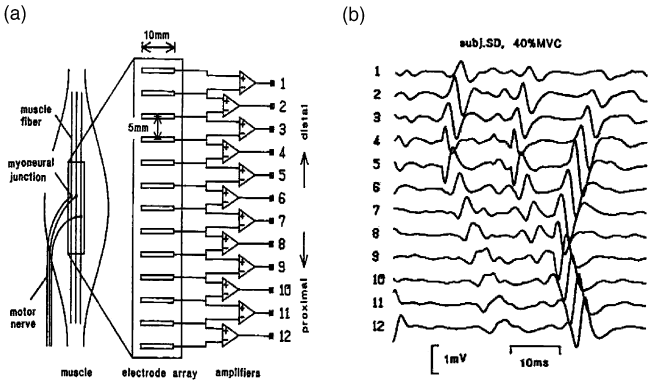
\includegraphics[width=\textwidth]{img/emg_array.png}
\end{figure}
\end{frame}

% CLASSIFICATION OF SIGNALS
\begin{frame}{Classification of signals (Contd ...)}
\begin{itemize}
\item \textbf{Deterministic} vs. \textbf{Stochastic}: \textit{e.g. EMG is an example of a stochastic signal.}
\end{itemize}
\begin{figure}
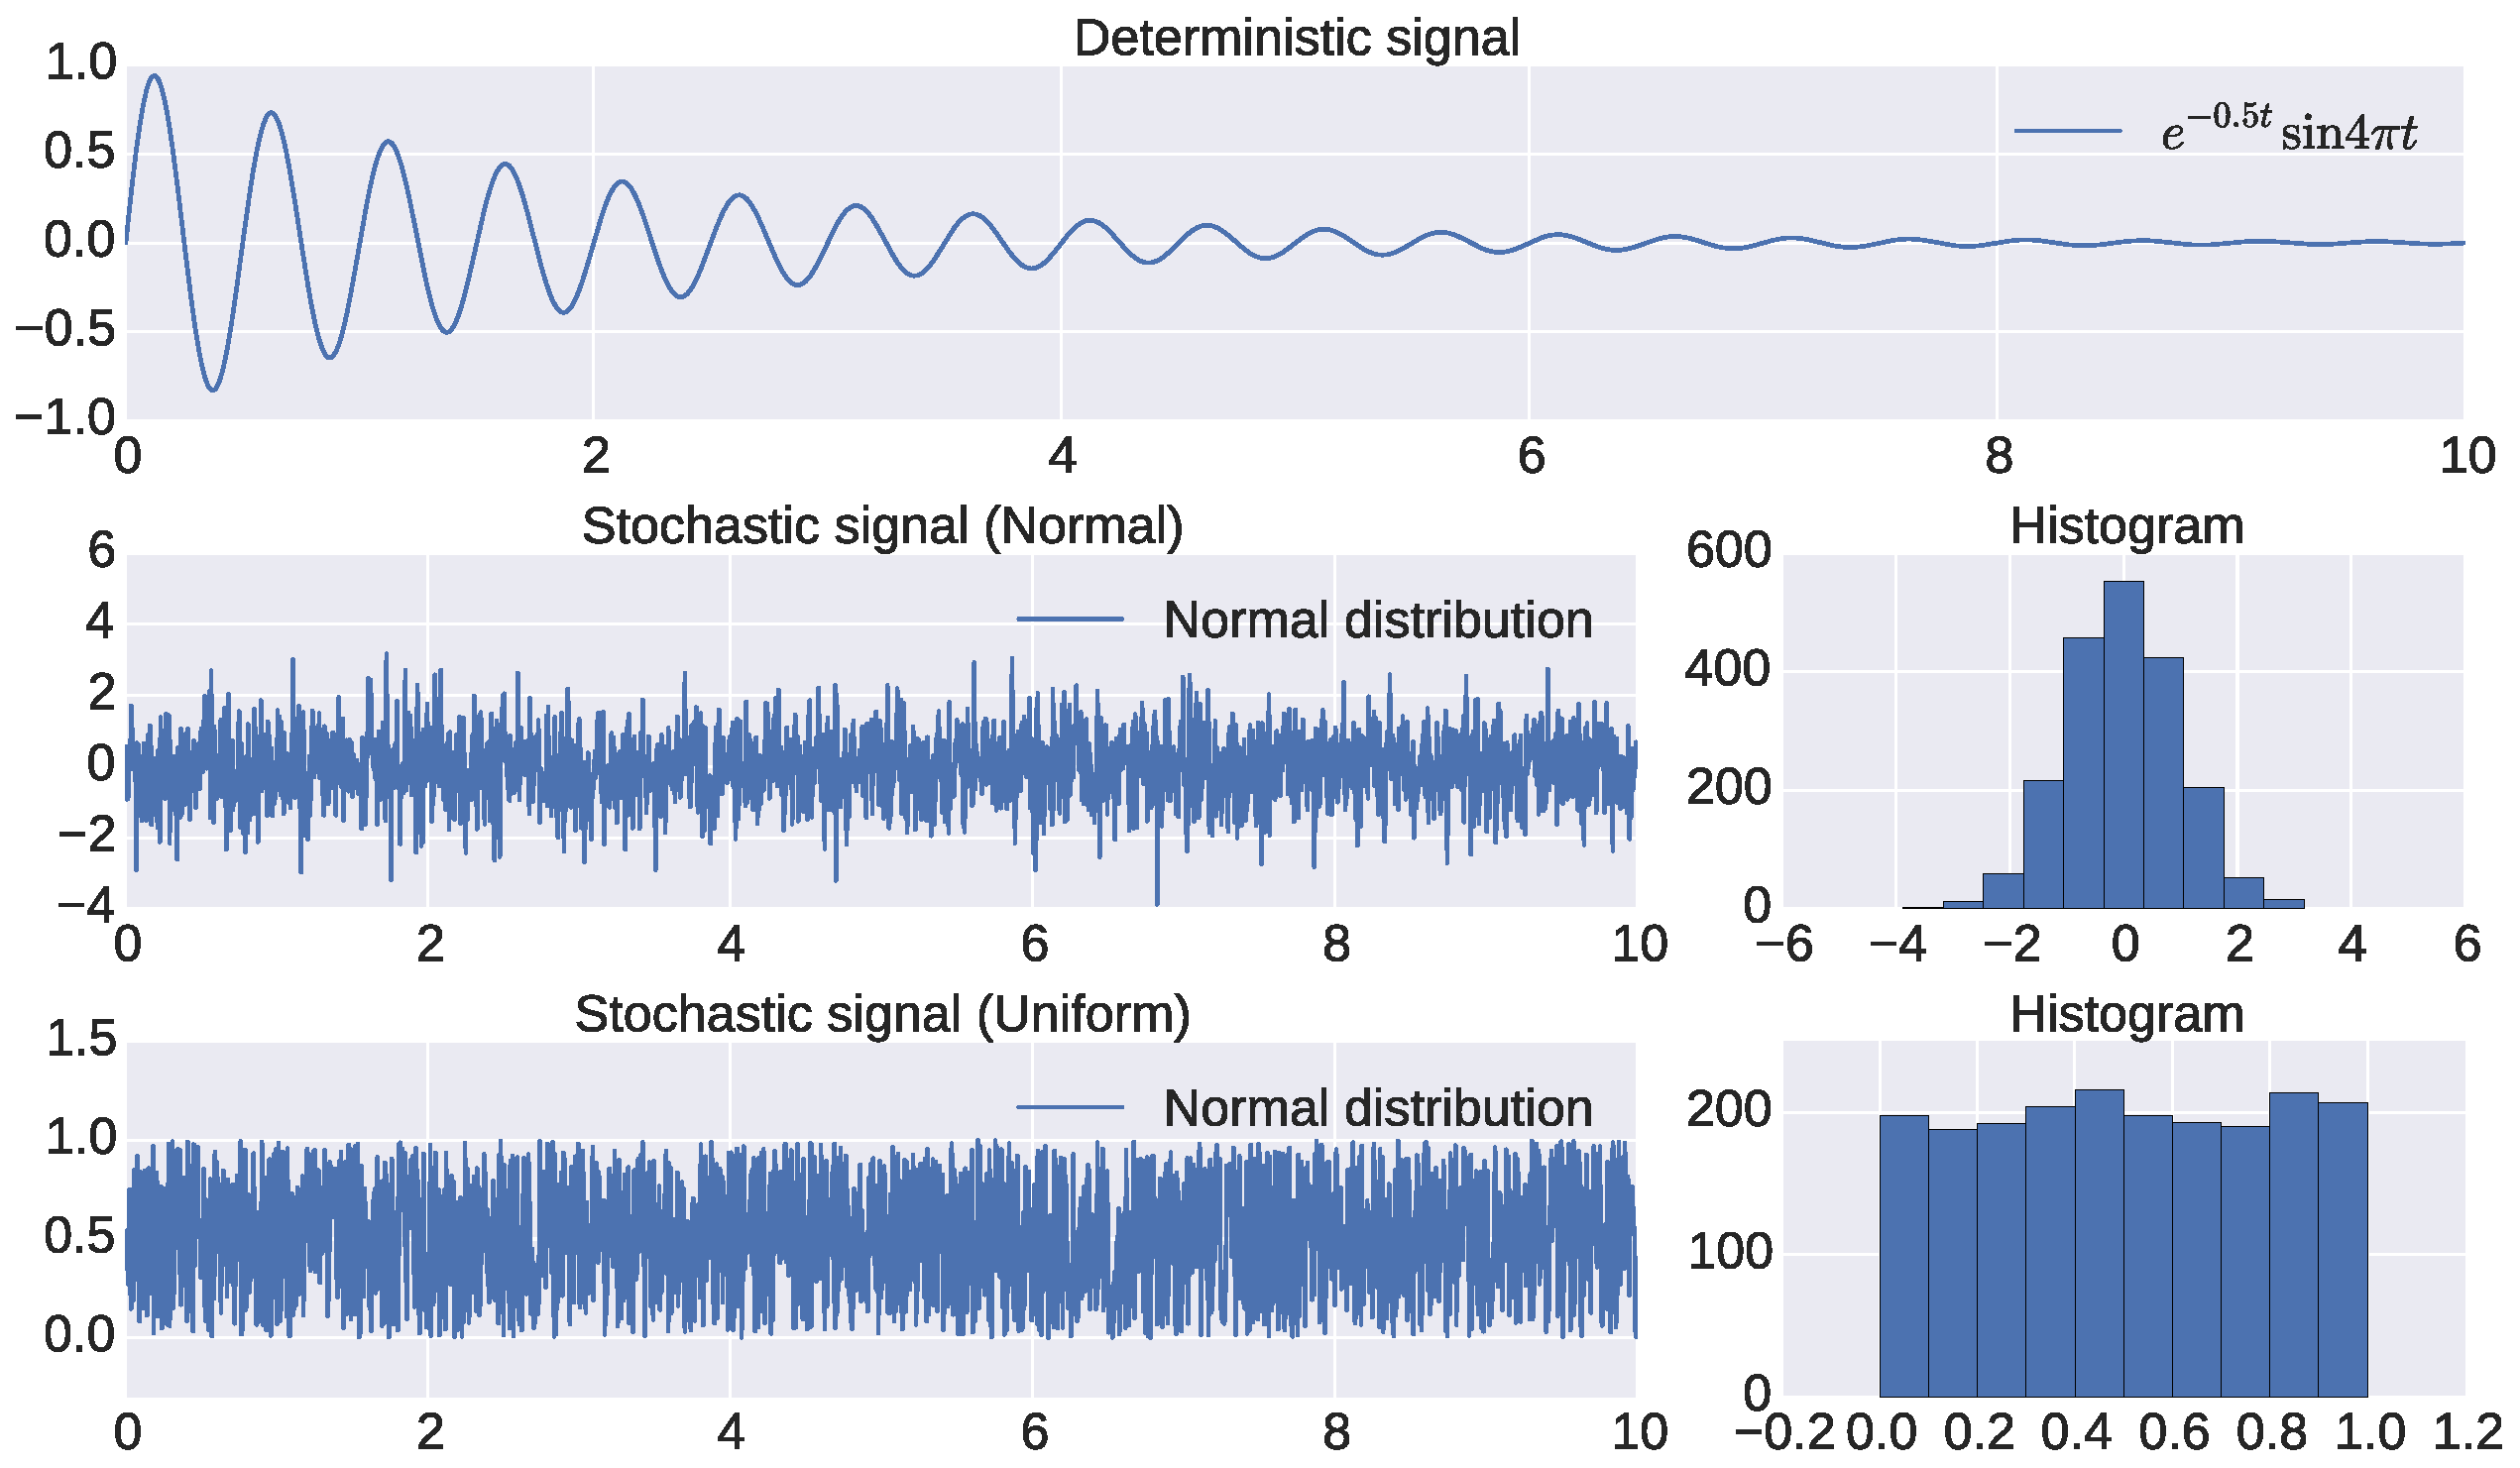
\includegraphics[width=\textwidth]{img/det_stoch.eps}
\end{figure}
\end{frame}

% CLASSIFICATION OF SIGNALS
\begin{frame}{Classification of signals (Contd ...)}
\begin{itemize}
\item \textbf{Even} vs. \textbf{Odd}: \textit{based on the symmetry about the} $t=0$ \textit{axis}.
\[\begin{cases}
x(t) = x(-t), & \text{Even signal} \\
x(t) = -x(-t), & \text{Odd signal} \\
\end{cases}\]

\textit{Can there be signals that are neither even nor odd?}

\begin{tcolorbox}[width=0.9\textwidth,colback={lightgray},title={\textbf{Theorem}},colbacktitle=black,coltitle=white]
\textit{Any arbitrary function can be represented as a sum of an odd and even function.}
\[ x(t) = x_{even}(t) + x_{odd}(t) \]
where, $ x_{even}(t) = \frac{x(t) + x(-t)}{2} $ and $ x_{odd}(t) = \frac{x(t) - x(-t)}{2} $.
\end{tcolorbox}
\end{itemize}
\end{frame}

% CLASSIFICATION OF SIGNALS
\begin{frame}{Classification of signals (Contd ...)}
\textbf{Decomposition of an arbitrary signal into even and odd components}
\begin{figure}
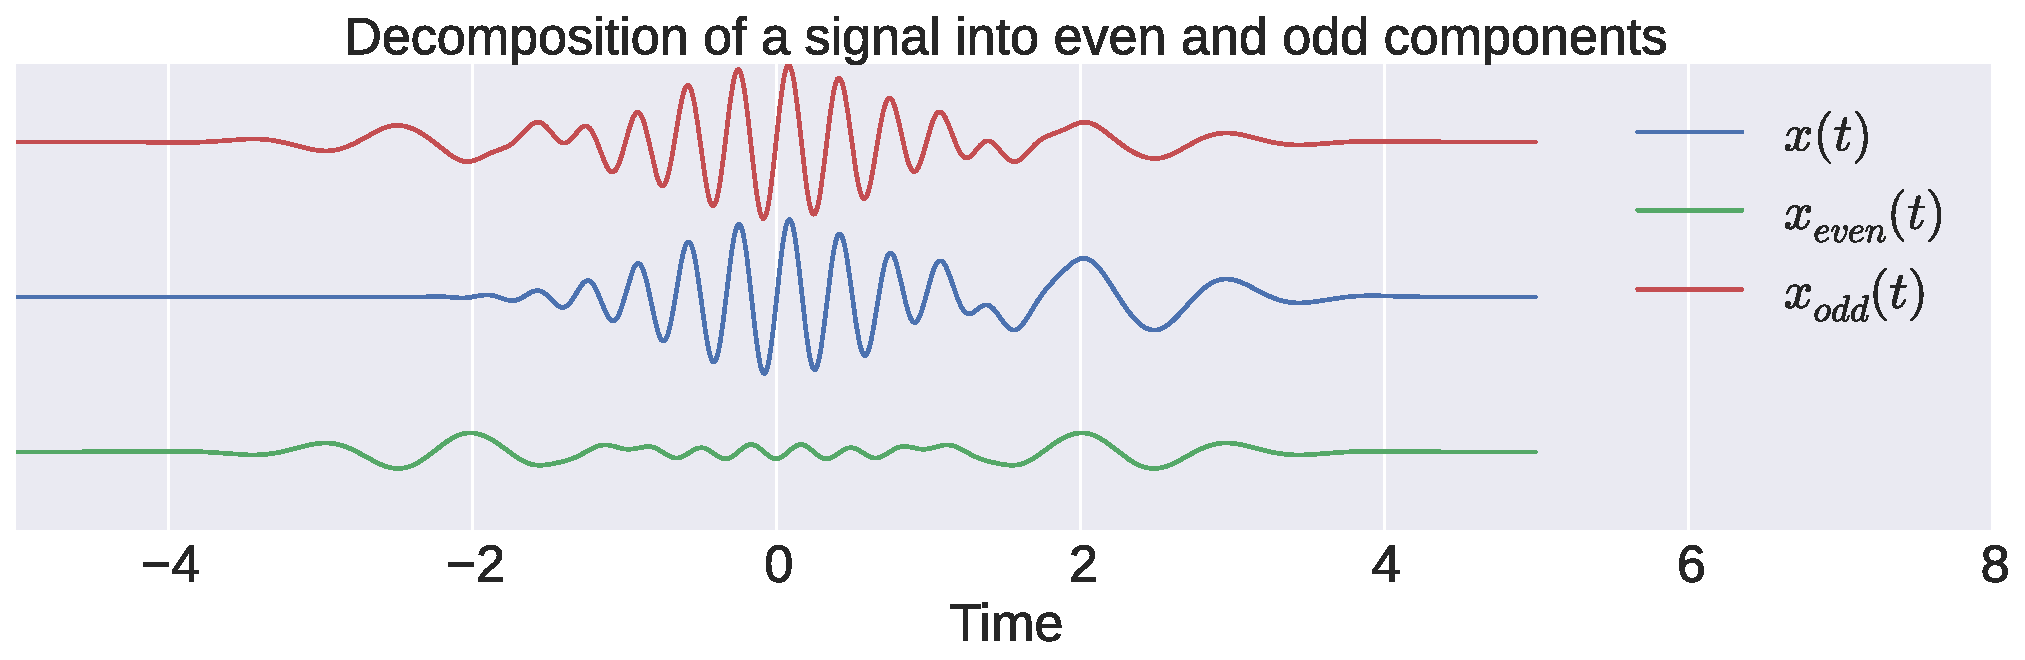
\includegraphics[width=\textwidth]{img/even_odd.eps}
\end{figure}
\end{frame}

% CLASSIFICATION OF SIGNALS
\begin{frame}{Classification of signals (Contd ...)}
\begin{itemize}
\item \textbf{Periodic} vs. \textbf{Non-periodic}: \textit{a signal is periodic, if and only if}
\[x\left(t\right) = x\left(t + T\right), \forall t\]
where, $T$ is the fundamental period.
\item \textbf{Energy} vs. \textbf{Power}: \textit{indicates if a signal is short-lived.}

\[ E = \int_{-\infty}^{\infty}\left|x(t)\right|^2dt \,\,\,\,\,\,\,\,\,\, P=\frac{1}{T}\int_{-T/2}^{T/2}\left|x(t)\right|^2dt \]

\[ E = \sum_{-\infty}^{\infty}\left|x(t)\right|^2 \,\,\,\,\,\,\,\,\,\, P=\frac{1}{2N+1}\sum_{-N}^{N}\left|x(t)\right|^2 \]

\textit{A signal is an \textbf{energy} signal, if} $0 < E < \infty$.

\textit{A signal is an \textbf{power} signal, if} $0 < P < \infty$.
\end{itemize}
\end{frame}

% WHAT IS A SYSTEM?
\begin{frame}{What is a system?}

A collection of objects united by some form of interaction or interdependence\footnote{Zadeh, Lotfi A., and Charles A. Deoser. \textit{Linear system theory}. New York: McGraw Hill, 1963.}.

\vspace{4mm}

From the signal processing point of view, \textbf{a system is any physical device or algorithm that performs some operation on a signal to transform it into another signal.}

\begin{figure}
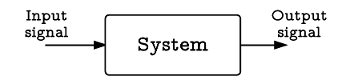
\includegraphics[width=0.7\textwidth]{img/system.png}
\end{figure}

Can be thought of a mapping function. \textit{e.g.}
\[ y = f\left(x\right) = kx \]

\end{frame}

% CLASSIFICATION OF SYSTEMS
\begin{frame}{Classification of systems}

Based on the properties of the system.

\begin{itemize}
\item \textbf{Linearity}: \textit{satisfies the properties of \textbf{scaling} and \textbf{superposition}}.

Let us assume, 
\[ f: x_i(t) \mapsto y_i(t) \]

The system $f$ is linear, if and only if,
\[ f:\sum_ia_ix_i(t) \mapsto \sum_ia_iy_i(t) \]

\textit{Which of these systems are linear?}
\begin{enumerate}
\item $y(t) = k_1x(t) + k_2x(t-2)$
\item $y(t) = \int_{t-T}^{t}x(\tau)d\tau$
\item $y(t) = 0.5x(t) + 1.5$
\end{enumerate}
\end{itemize}
\end{frame}

% CLASSIFICATION OF SYSTEMS
\begin{frame}{Classification of systems}

Based on the properties of the system.

\begin{itemize}
\item \textbf{Memory}: \textit{a system whose output depends on past or future values of its input is a system with memory, else the system is memoryless}. 

Note: the system may or may not depends on its present.

\[ \begin{cases}
y(t) = 0.5x(t) & \mathrm{\textbf{Memoryless system}} \\
y(t) = \int_{t-0.5}^{t}x(\tau)d\tau & \mathrm{\textbf{System with memory}}
\end{cases}
\]
\end{itemize}

\begin{figure}
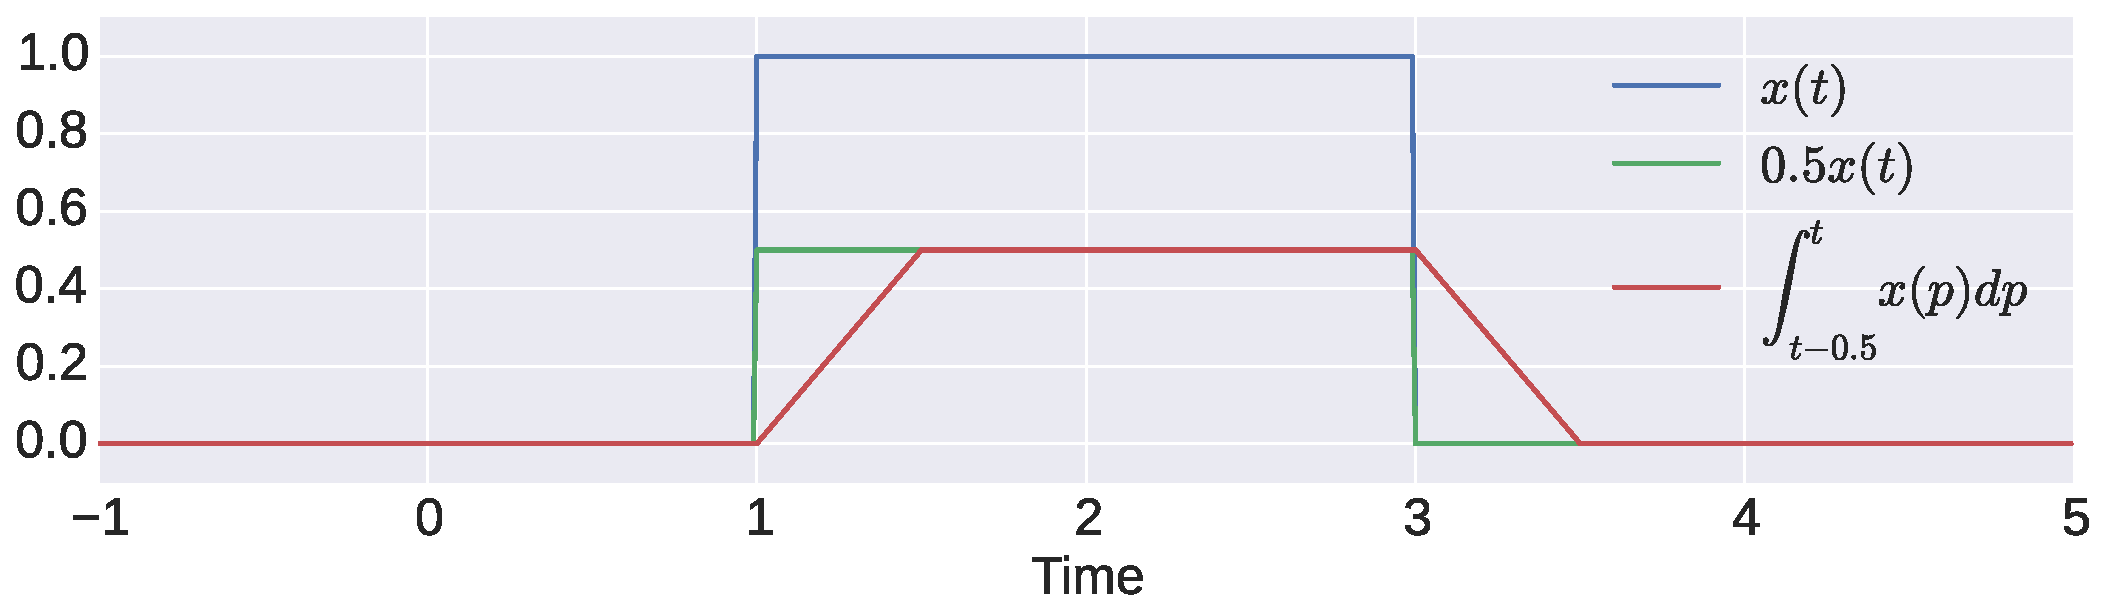
\includegraphics[width=0.7\textwidth]{img/memory.eps}
\end{figure}

\end{frame}

% CLASSIFICATION OF SYSTEMS
\begin{frame}{Classification of systems}

\begin{itemize}
\item \textbf{Causality}: \textit{a system whose output depends on the past and present only values of the input is a causal system}.
\[ \begin{cases}
y(t) = \int_{t-0.5}^{t}x(\tau)d\tau & \mathrm{\textbf{Causal}} \\
y(t) = \int_{t-0.5}^{t+0.5}x(\tau)d\tau & \mathrm{\textbf{Non-causal}}
\end{cases}
\]

\item \textbf{Time invariance}: \textit{system remains the same with time}.

If s system is time-invariant, then
\[ f:x\left(t\right) \mapsto y\left(t\right) \iff f:x\left(t-t_0\right) \mapsto y\left(t-t_0\right)\]

\item \textbf{Stability}: \textit{bounded input produces bounded output}.

\[ \left|x\left(t\right)\right| < M_x < \infty \mapsto \left|y\left(t\right)\right| < M_y < \infty \]

\item \textbf{Invertibility}: \textit{input can be recovered from output}.
\end{itemize}
\end{frame}

\end{document}


